\clearpage
\section{Endoscopic Polypectomy and Colorectal Polyps}
\label{sec:polypectomy}
\subsection{What is a Polyp?}
A \textbf{colorectal polyp} is an abnormal growth from the lining of the colon or rectum. It can be small and flat or larger and on a stalk. The most common precancerous type is called an \textbf{adenoma}, which is a glandular polyp with a higher risk of becoming cancer over time, so it is often removed during colonoscopy even when it does not yet cause symptoms.

This is why polyp size, shape, and appearance matter in practice: the endoscopist has to decide quickly whether the lesion should be removed and how much risk is involved.


\begin{figure}[H]
\centering
\setlength{\fboxsep}{4pt}% padding for frame
\fbox{%
	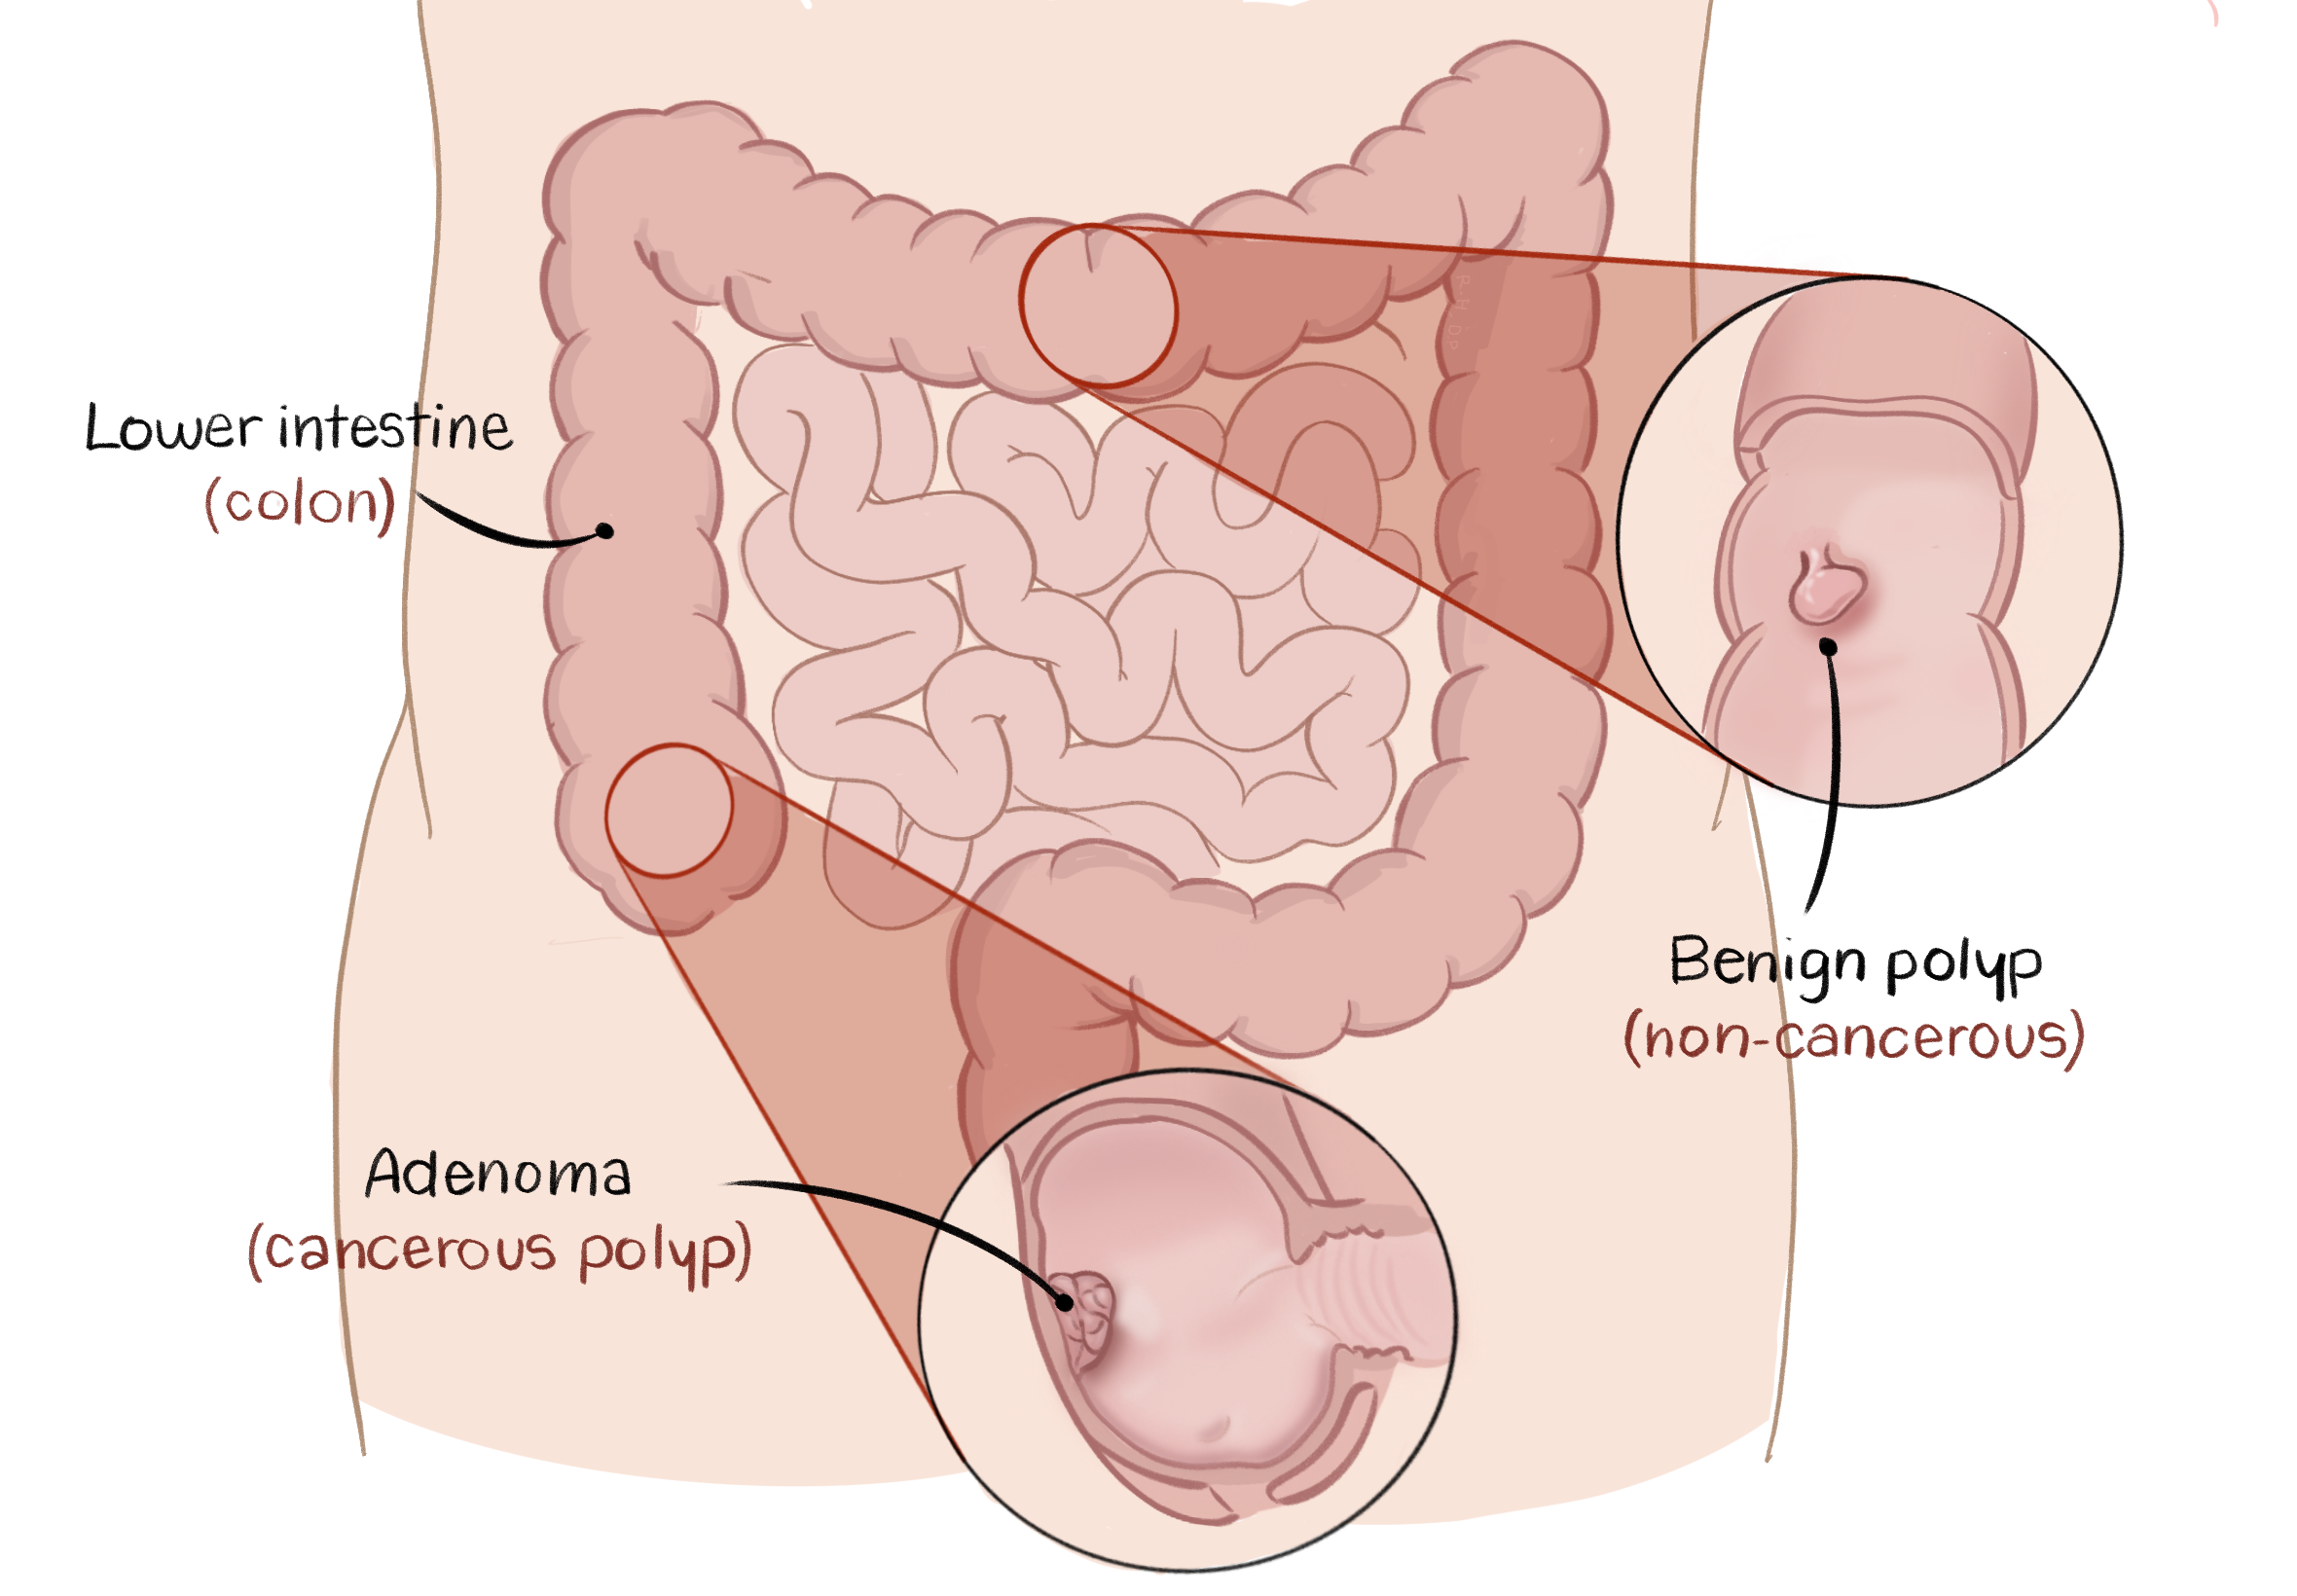
\includegraphics[width=1\linewidth,trim=0cm 0cm 1cm 0cm,clip]{assets/illustration-colon-polyps.png}%
}
\caption{Illustration of polyps inside the colon.}
\label{fig:colon_polyps}
\end{figure}

After removal, polyps are sent for \textbf{histology} to check for cancer or high‑risk features. \textbf{Small polyps} are often removed during the same colonoscopy, while larger or complex lesions may need \textbf{advanced techniques} or referral. The choice balances \textbf{completeness} of removal and patient \textbf{safety}.

\begin{figure}[H]
\centering
\setlength{\fboxsep}{4pt}% padding for frame
\fbox{%
	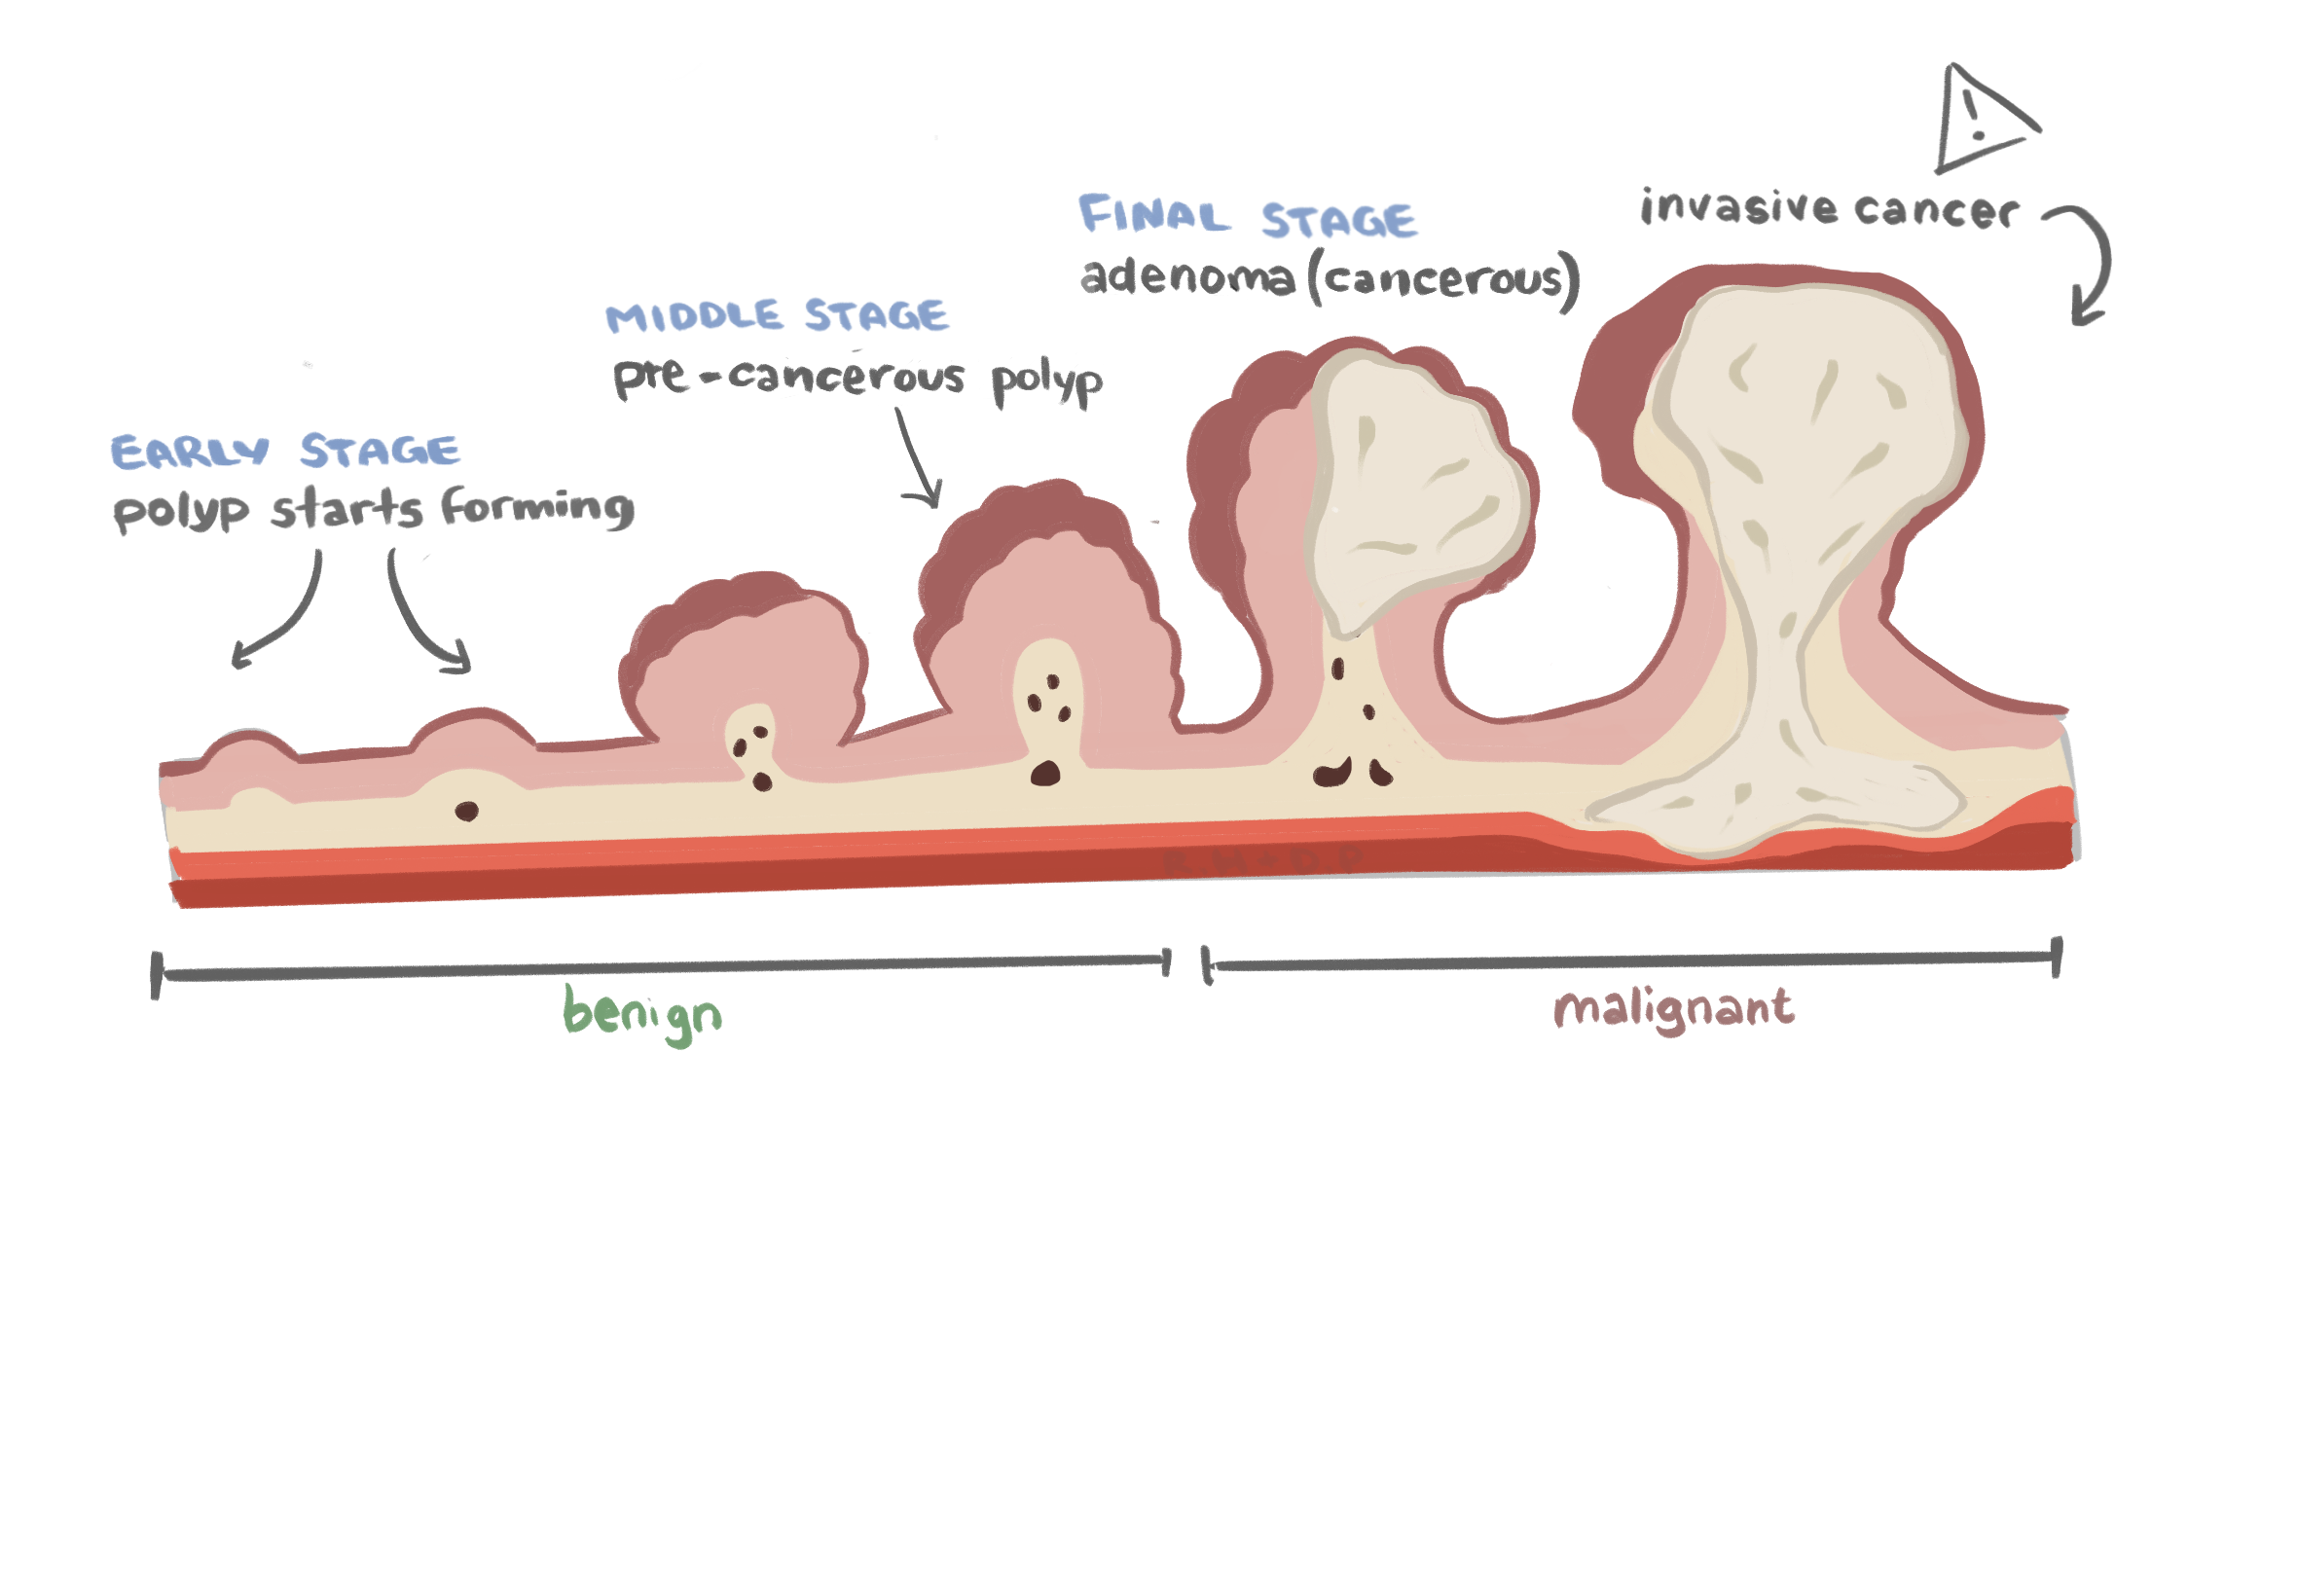
\includegraphics[width=1\linewidth,trim=1cm 6cm 2cm 4cm,clip]{assets/illustration-polyp-growth.png}%
}
\caption{Illustration of a colorectal polyp (growth stages).}
\label{fig:colorectal_polyp}
\end{figure}

Colorectal polyps are very common. Studies show that about \textbf{25--30\,\%} of adults over 50 have at least one adenomatous polyp, and this number goes up to \textbf{40--50\,\%} by age 70 \cite{strum2016prevalence}. Most polyps are small, usually under \textbf{10\,mm}, and they do not cause any symptoms. However, a small number of them follow the \textbf{adenoma to carcinoma sequence}, which is a step-by-step process where normal tissue slowly turns into cancer over \textbf{10--15 years} \cite{leslie2024polyps}. Because this process takes so long, screening is very useful since it gives doctors a wide window to find and remove polyps before they become dangerous.

The effect of removing polyps is significant. The well-known \textbf{National Polyp Study} showed that polypectomy during colonoscopy can reduce the chance of getting colorectal cancer by \textbf{76--90\,\%} \cite{winawer1993polypectomy}. Other research found that for every \textbf{1\,\%} increase in a doctor's \textbf{adenoma detection rate} (ADR), there is a \textbf{3\,\%} drop in the risk of colorectal cancer appearing later \cite{corley2014adr}. Because of this, the ADR is now used as a quality measure, and guidelines say it should be at least \textbf{25\,\%} \cite{lieberman2014screening}. Even so, studies estimate that around \textbf{26\,\%} of adenomas are still \textit{missed} during a normal examination, especially flat and right-sided ones \cite{zhao2019adenomaMiss}.

Looking at the bigger picture, colorectal cancer is the \textbf{third most common} cancer in the world and the \textbf{second leading} cause of cancer death. In 2022 alone, there were about \textbf{1.9 million} new cases and \textbf{900\,000} deaths \cite{iarc2024globocan,sung2021globocan}. These numbers show why organised screening programmes are so important. In countries like the UK, Germany, and parts of the US where screening is well established, polypectomy has helped reduce colorectal cancer deaths over time.

\clearpage
\subsection{What is an Endoscope?}
An \textbf{endoscope} is a long, flexible tube with a tiny camera and a light at the tip. Doctors use it to look inside the body without making any cuts. During a colonoscopy, the endoscope goes in through the rectum and moves along the colon so the doctor can check the inner lining for anything unusual, like polyps. It also has small channels inside that let the doctor pass tools such as snares or forceps to take samples or remove lesions. Controlling the scope, the camera angle, and the tools all at the same time is quite difficult and needs a lot of practice.

\begin{figure}[H]
\centering
\setlength{\fboxsep}{4pt}
\fbox{%
	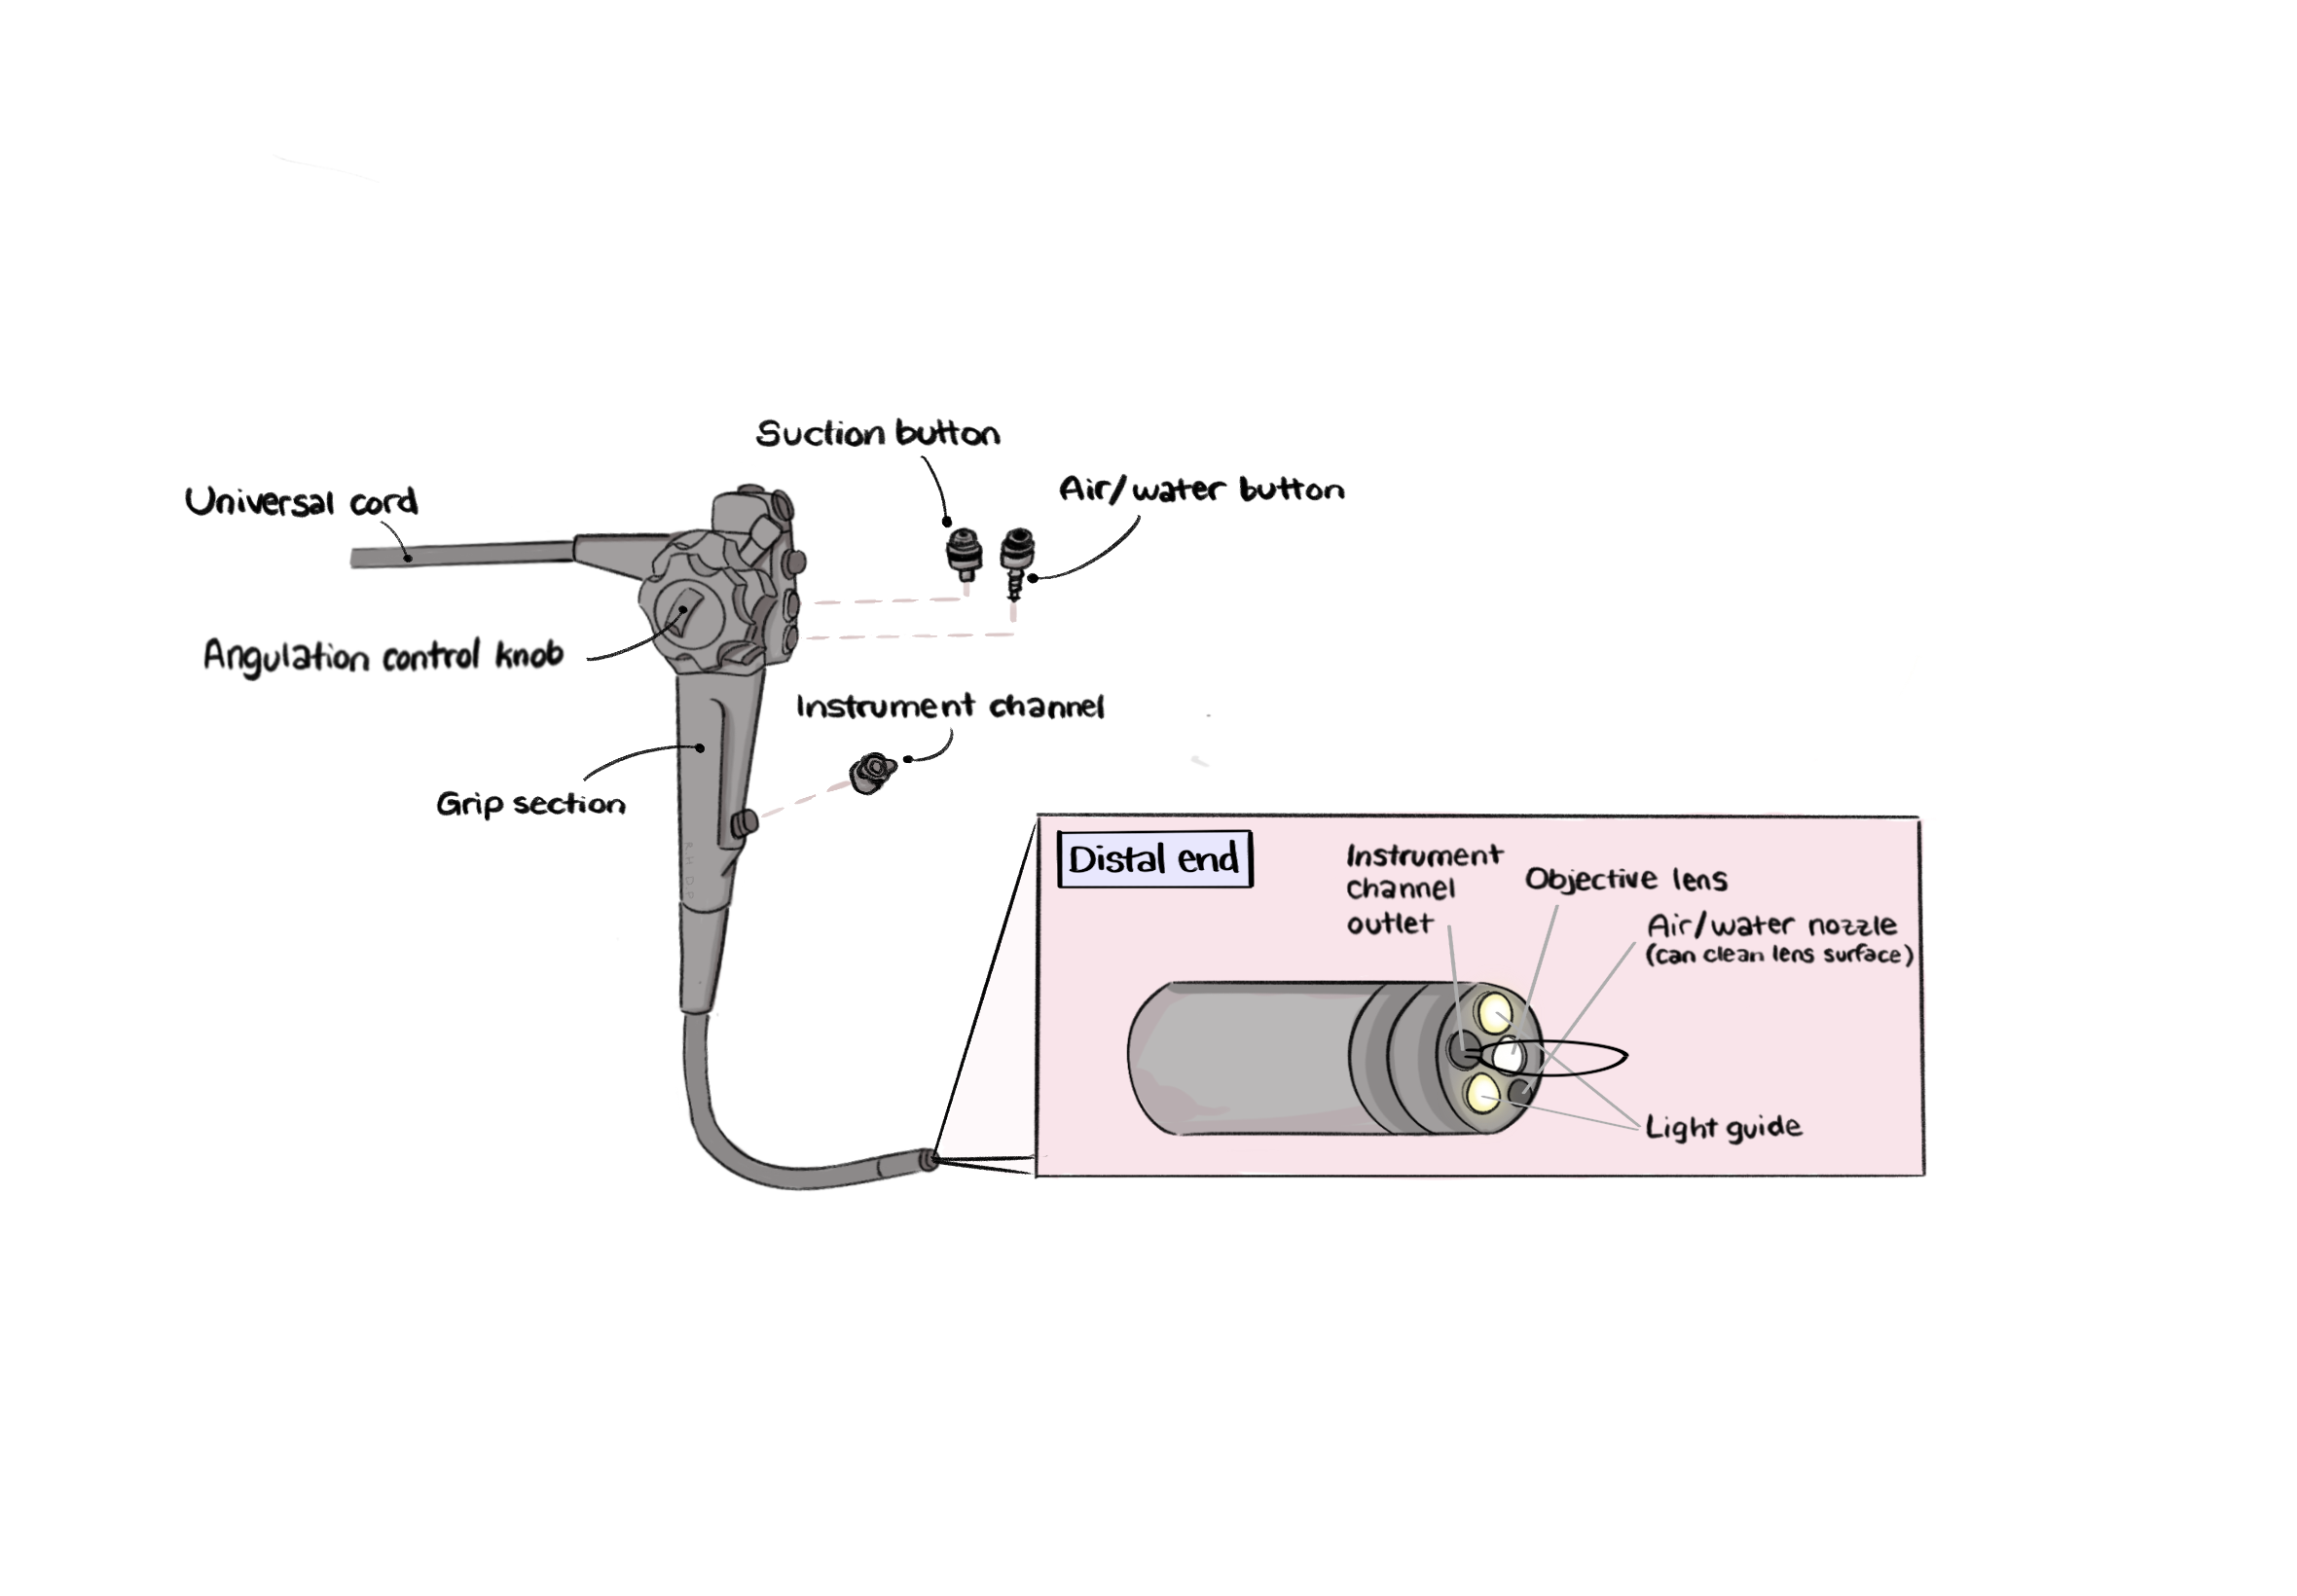
\includegraphics[width=1\linewidth,trim=2cm 6cm 6cm 5cm,clip]{assets/illustration-endoscope.png}%
}
\caption{Endoscope Components.}
\label{fig:endoscope_components}
\end{figure}

A modern endoscope provides a \textbf{live video feed} in high definition. The operator can bend the tip using \textbf{tip deflection} controls to get the best viewing angle. Other useful features include \textbf{insufflation}, which blows air or CO\textsubscript{2} to open up the colon walls, and \textbf{suction} to clear any fluid that blocks the view. The \textbf{instrument channel} allows the doctor to insert different tools depending on what needs to be done. Good \textbf{image quality} and a steady hand make it much easier to spot small polyps and treat them safely.

\begin{figure}[H]
\centering
\setlength{\fboxsep}{4pt}
\fbox{%
	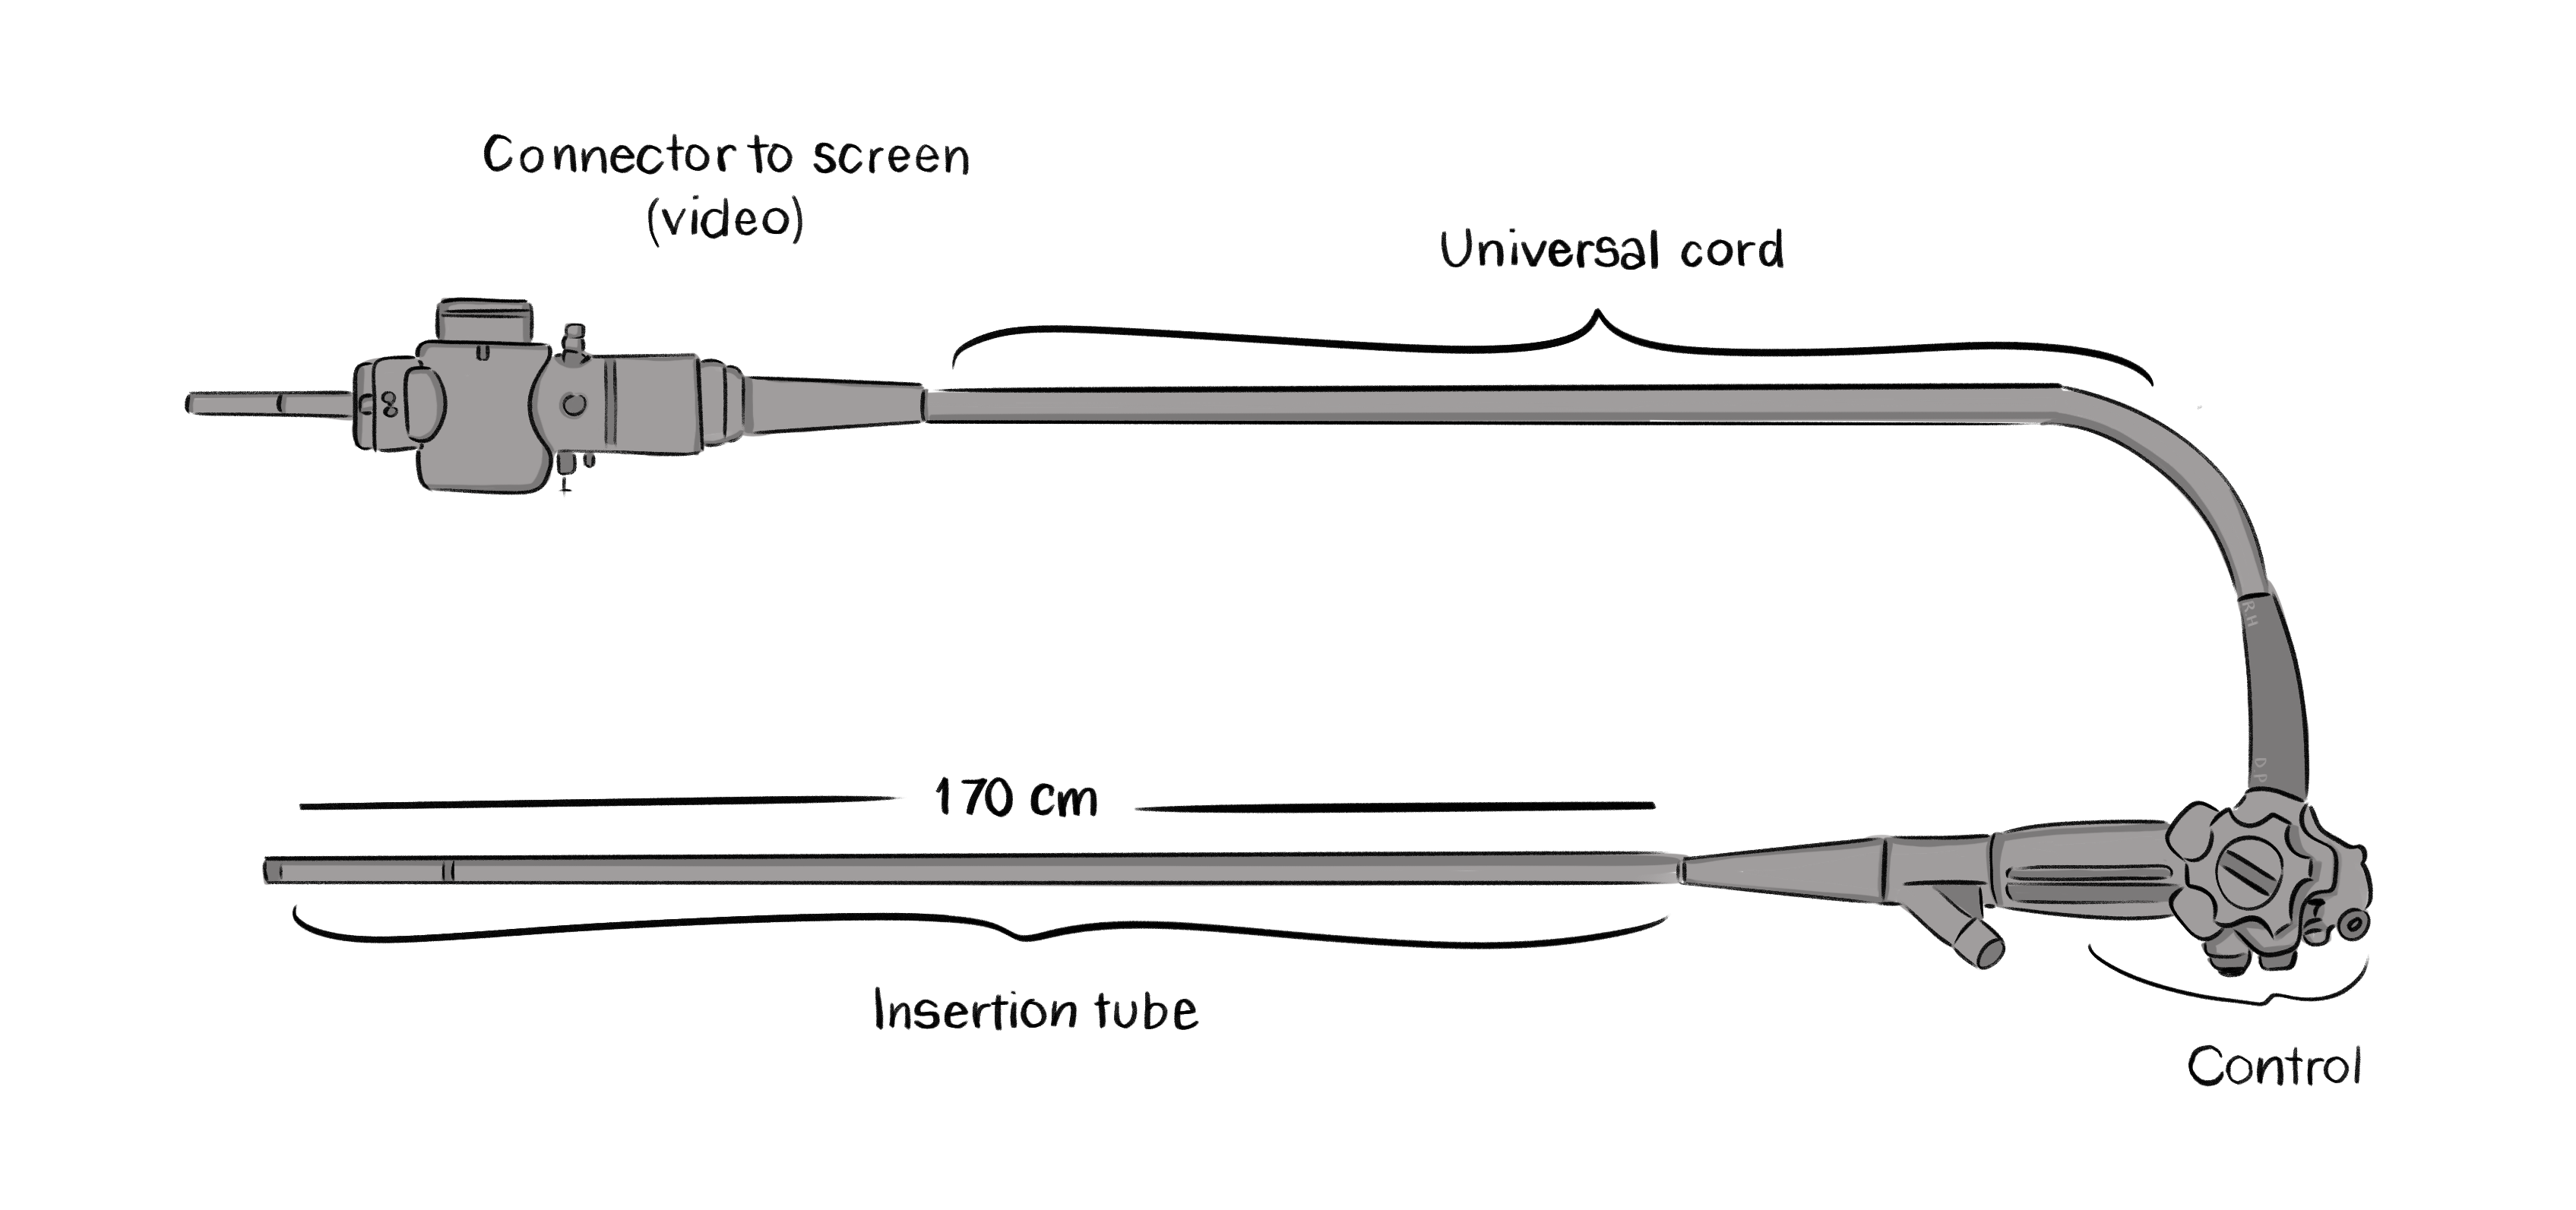
\includegraphics[width=1\linewidth]{assets/illustration-endoscope-dimensions.png}%
}
\caption{Endoscope Dimensions.}
\label{fig:endoscope_dimensions}
\end{figure}

The physical design of the endoscope is a careful balance between reach, flexibility, and patient comfort. The \textbf{insertion tube} is usually \textbf{130 to 170\,cm} long, which is enough to reach the full length of the colon. However, a longer tube can sometimes form loops inside the body, making it harder to control \cite{ferlitsch2017esge}. The \textbf{outer diameter} is typically \textbf{9 to 13\,mm}, and thinner scopes are more comfortable for the patient but may limit the size of instruments that can be used. The \textbf{working channel} (about \textbf{2.8 to 3.8\,mm} wide) decides which tools can fit through, such as snares, biopsy forceps, or retrieval nets. The \textbf{bending section} at the tip can move in multiple directions, which is essential for getting a clear, stable view of the colon wall.

Other features worth mentioning are the \textbf{control section}, where the operator adjusts the tip angle and manages instruments, and the built-in channels for \textbf{insufflation} and \textbf{suction}. For AI-assisted systems, things like \textbf{image quality}, low \textbf{latency}, and a stable video feed are very important because the computer needs a clear and consistent picture to work well.

\clearpage
\subsection{What is Colonoscopy?}

A \textbf{colonoscopy} is a medical procedure where the doctor uses an endoscope to look inside the entire colon and rectum. It is one of the most common procedures in gastroenterology, with over \textbf{19 million} colonoscopies performed every year in the United States alone \cite{lieberman2014screening}. It is used for three main purposes: \textbf{screening} for cancer, \textbf{diagnosing} problems like bleeding or inflammation, and \textbf{treating} issues such as removing polyps. Before the procedure, the patient needs good \textbf{bowel preparation} so that the doctor can see the lining of the colon clearly.

The main steps are simple to understand: first the patient is \textbf{prepared} and given \textbf{light sedation}, then the scope is \textbf{inserted and pushed forward} until it reaches the \textbf{cecum} (the start of the colon). After that, the doctor slowly \textbf{pulls the scope back} while carefully checking the walls for any lesions. If something is found, it can be \textbf{sampled or removed} right away. The whole process usually takes about \textbf{20 to 40 minutes}. Two important quality measures are the \textbf{cecal intubation rate} (how often the doctor reaches the cecum) and the \textbf{adenoma detection rate} (how often adenomas are found) \cite{corley2014adr}.

\begin{figure}[H]
\centering
\setlength{\fboxsep}{4pt}
\fbox{%
	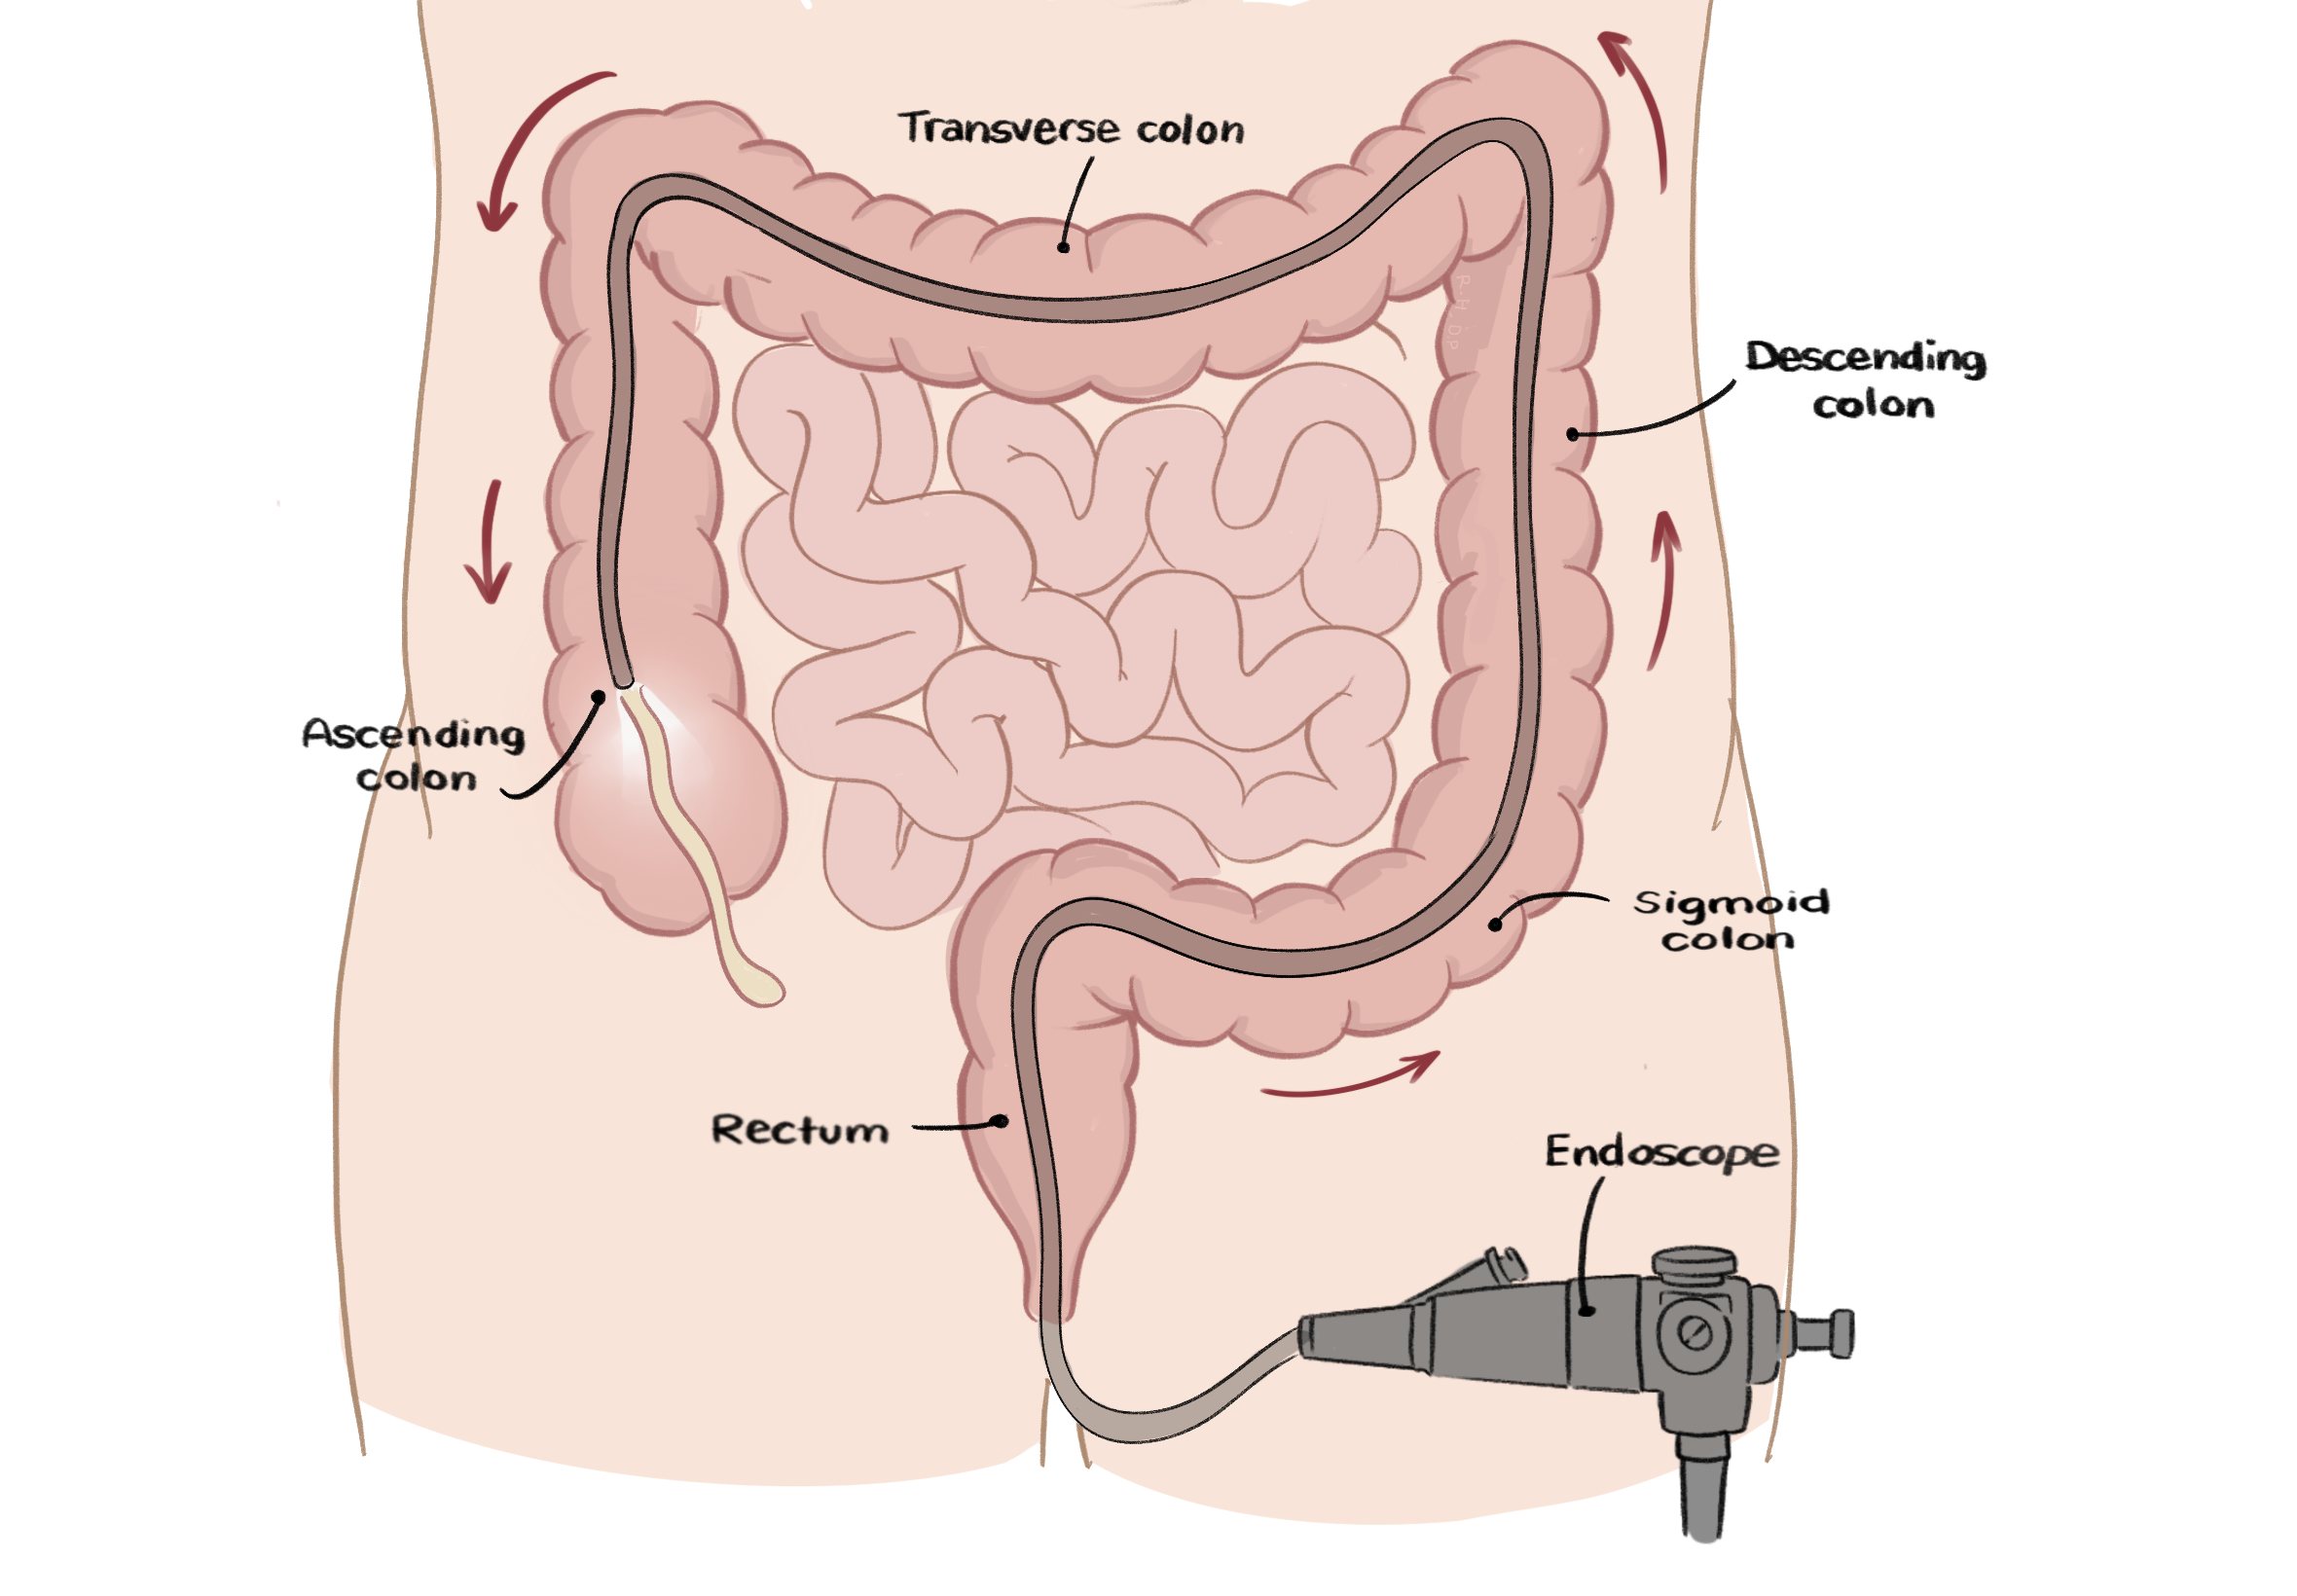
\includegraphics[width=1\linewidth,trim=1cm 0cm 2cm 0cm,clip]{assets/illustration-colonoscopy.png}%
}
\caption{Colonoscopy: scope view and instruments.}
\label{fig:colonoscopy_illustration}
\end{figure}

If a polyp is removed during the procedure, the doctor may use \textbf{clips} or \textbf{cautery} to stop any bleeding at the site. After the colonoscopy, the patient gets clear written instructions about what to watch for and when to come back. Follow-up depends on the \textbf{histology results} and the \textbf{size of the lesion} that was removed.

To put it simply: \textbf{endoscopy} is any procedure that uses a flexible camera to look inside the body. A \textbf{colonoscopy} is a specific type of endoscopy that examines the \textbf{colon} and \textbf{rectum}, and it is often done to screen for colorectal cancer or investigate symptoms. A \textbf{polypectomy} is when a \textbf{polyp} is actually removed during the colonoscopy.

\begin{figure}[H]
\centering
\setlength{\fboxsep}{4pt}
\fbox{%
	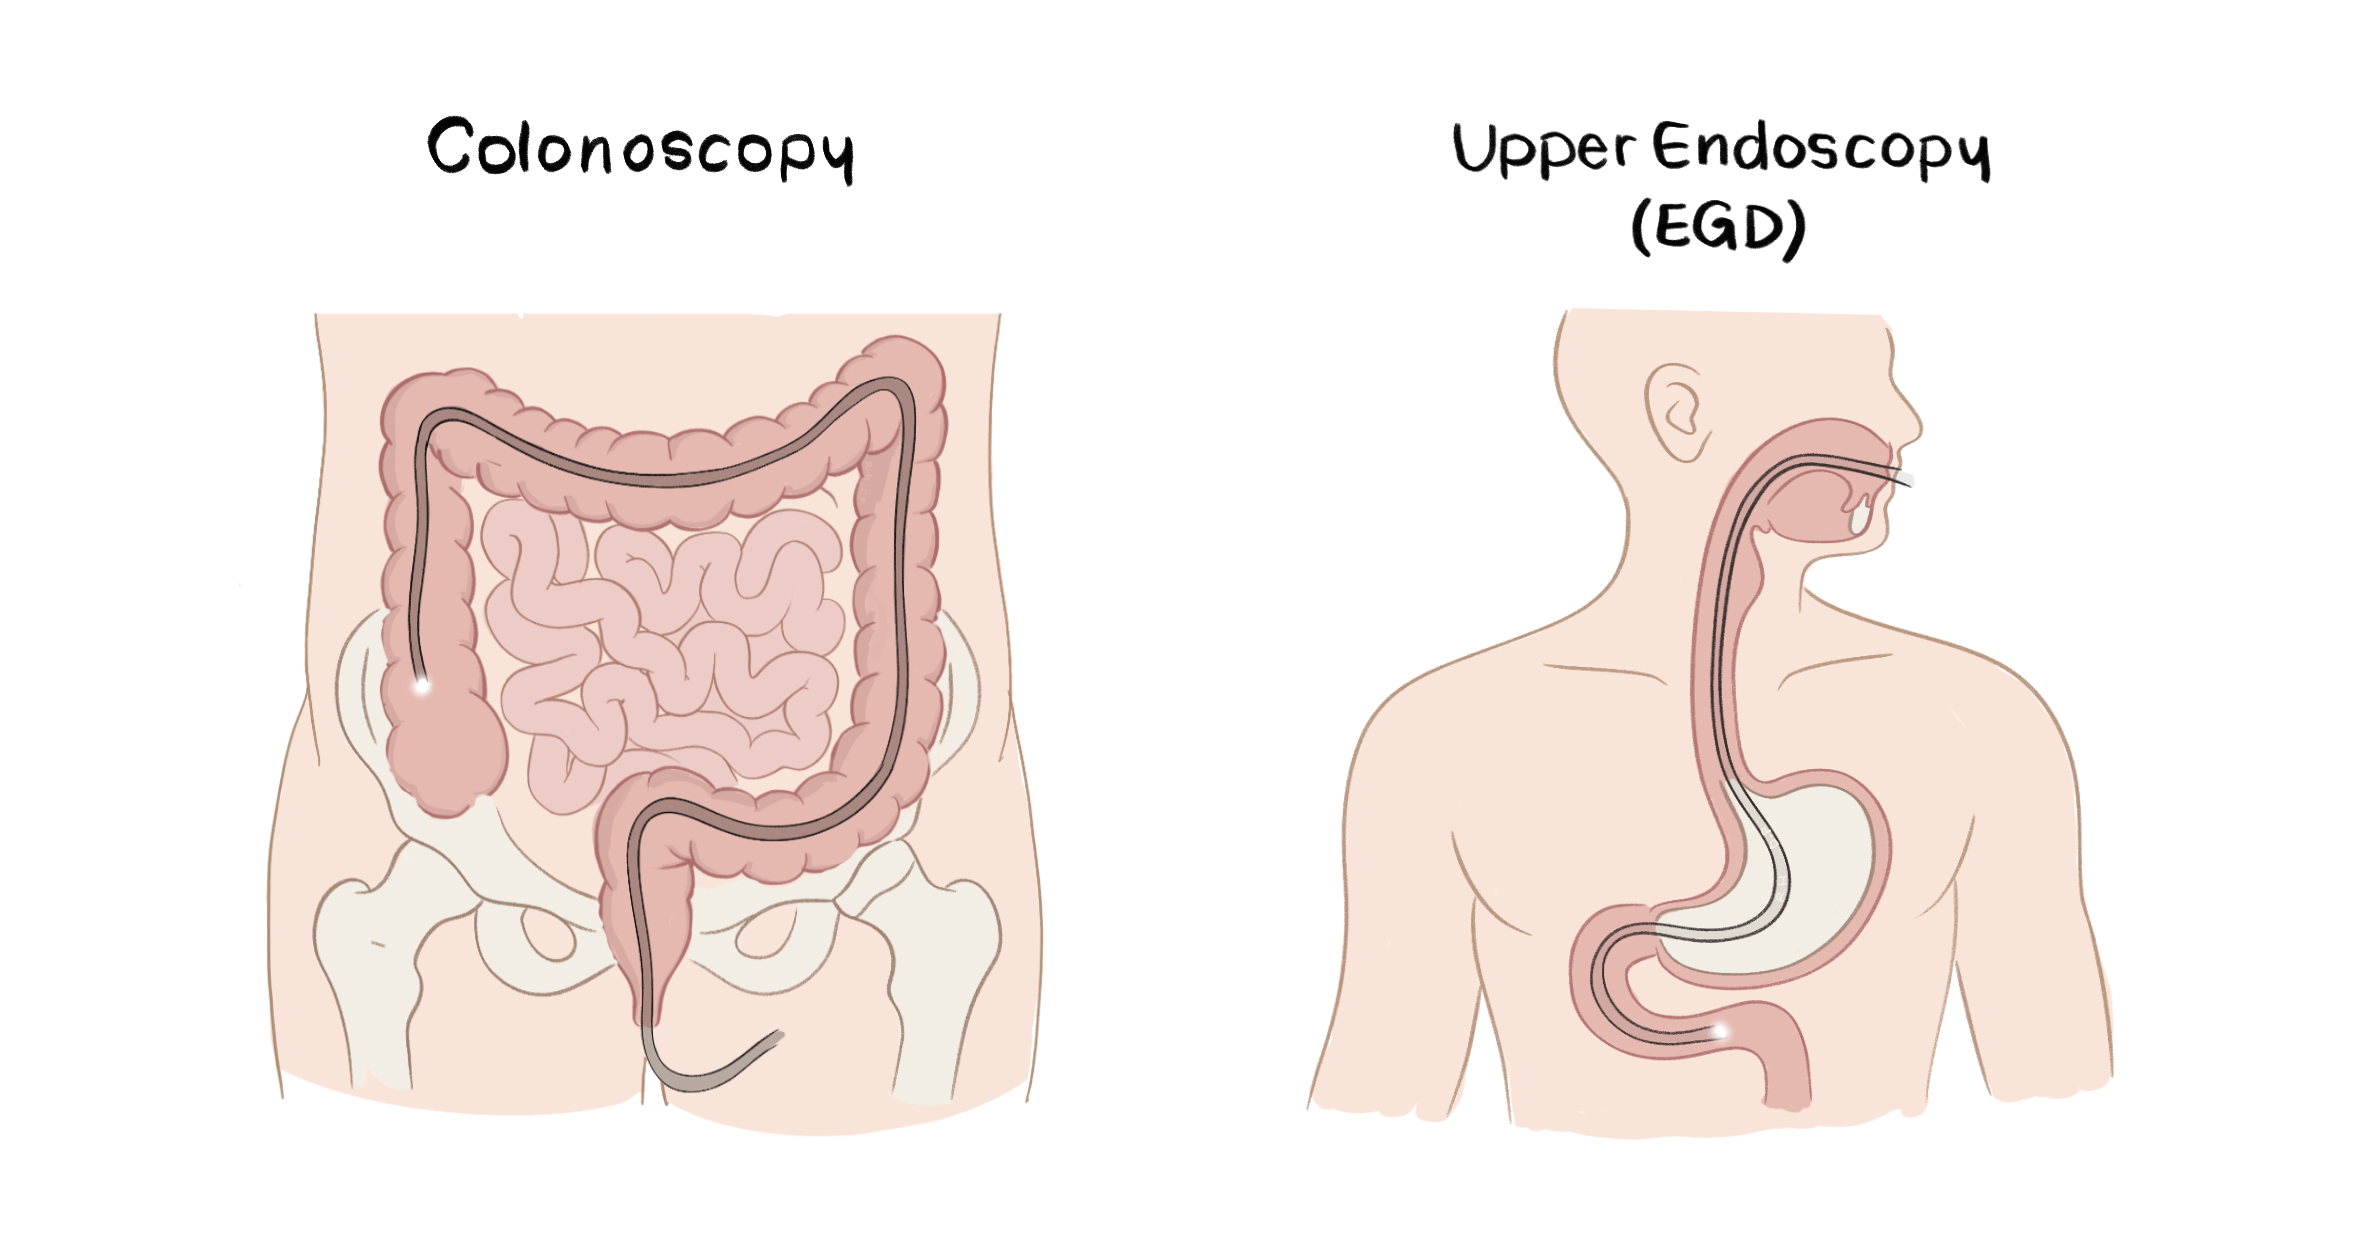
\includegraphics[width=1\linewidth]{assets/illustration-colonoscopy-vs-EGD.png}%
}
\caption{Colonoscopy vs Upper Endoscopy (EGD)}
\label{fig:colonoscopy_vs_upper-endoscopy}
\end{figure}

The abbreviation \textbf{EGD} stands for \textbf{EsophagoGastroDuodenoscopy}. Breaking it down: \textbf{Esophago} refers to the esophagus (the tube from the mouth to the stomach), \textbf{Gastro} refers to the stomach, \textbf{Duodeno} refers to the duodenum (the first part of the small intestine), and \textbf{-scopy} means looking or examining with a camera.


\clearpage
\subsection{What is Polypectomy?}
A \textbf{polypectomy} is the endoscopic \textbf{resection} (removal) of \textbf{colorectal polyps} during colonoscopy. Polyps may be benign, precancerous (\textbf{adenomas}), or malignant. Because appearance alone cannot exclude malignancy, \textbf{resection} and \textbf{histopathological assessment} are often recommended.

A \textbf{polypectomy} is therefore a subset of \textbf{endoscopy} - procedures that use an \textbf{endoscope} to visualise and sometimes treat the gastrointestinal tract.

Beyond screening, polypectomy is a \textbf{real-time} procedure that requires the operator to: \textbf{spot the lesion}, \textbf{judge its shape}, select the \textbf{resection method}, \textbf{position tools}, \textbf{manage bleeding risk}, and ensure the \textbf{removal is complete}. This is why reliable \textbf{perception} and safe \textbf{decision-making} are essential.

\begin{figure}[H]
\centering
\fbox{
	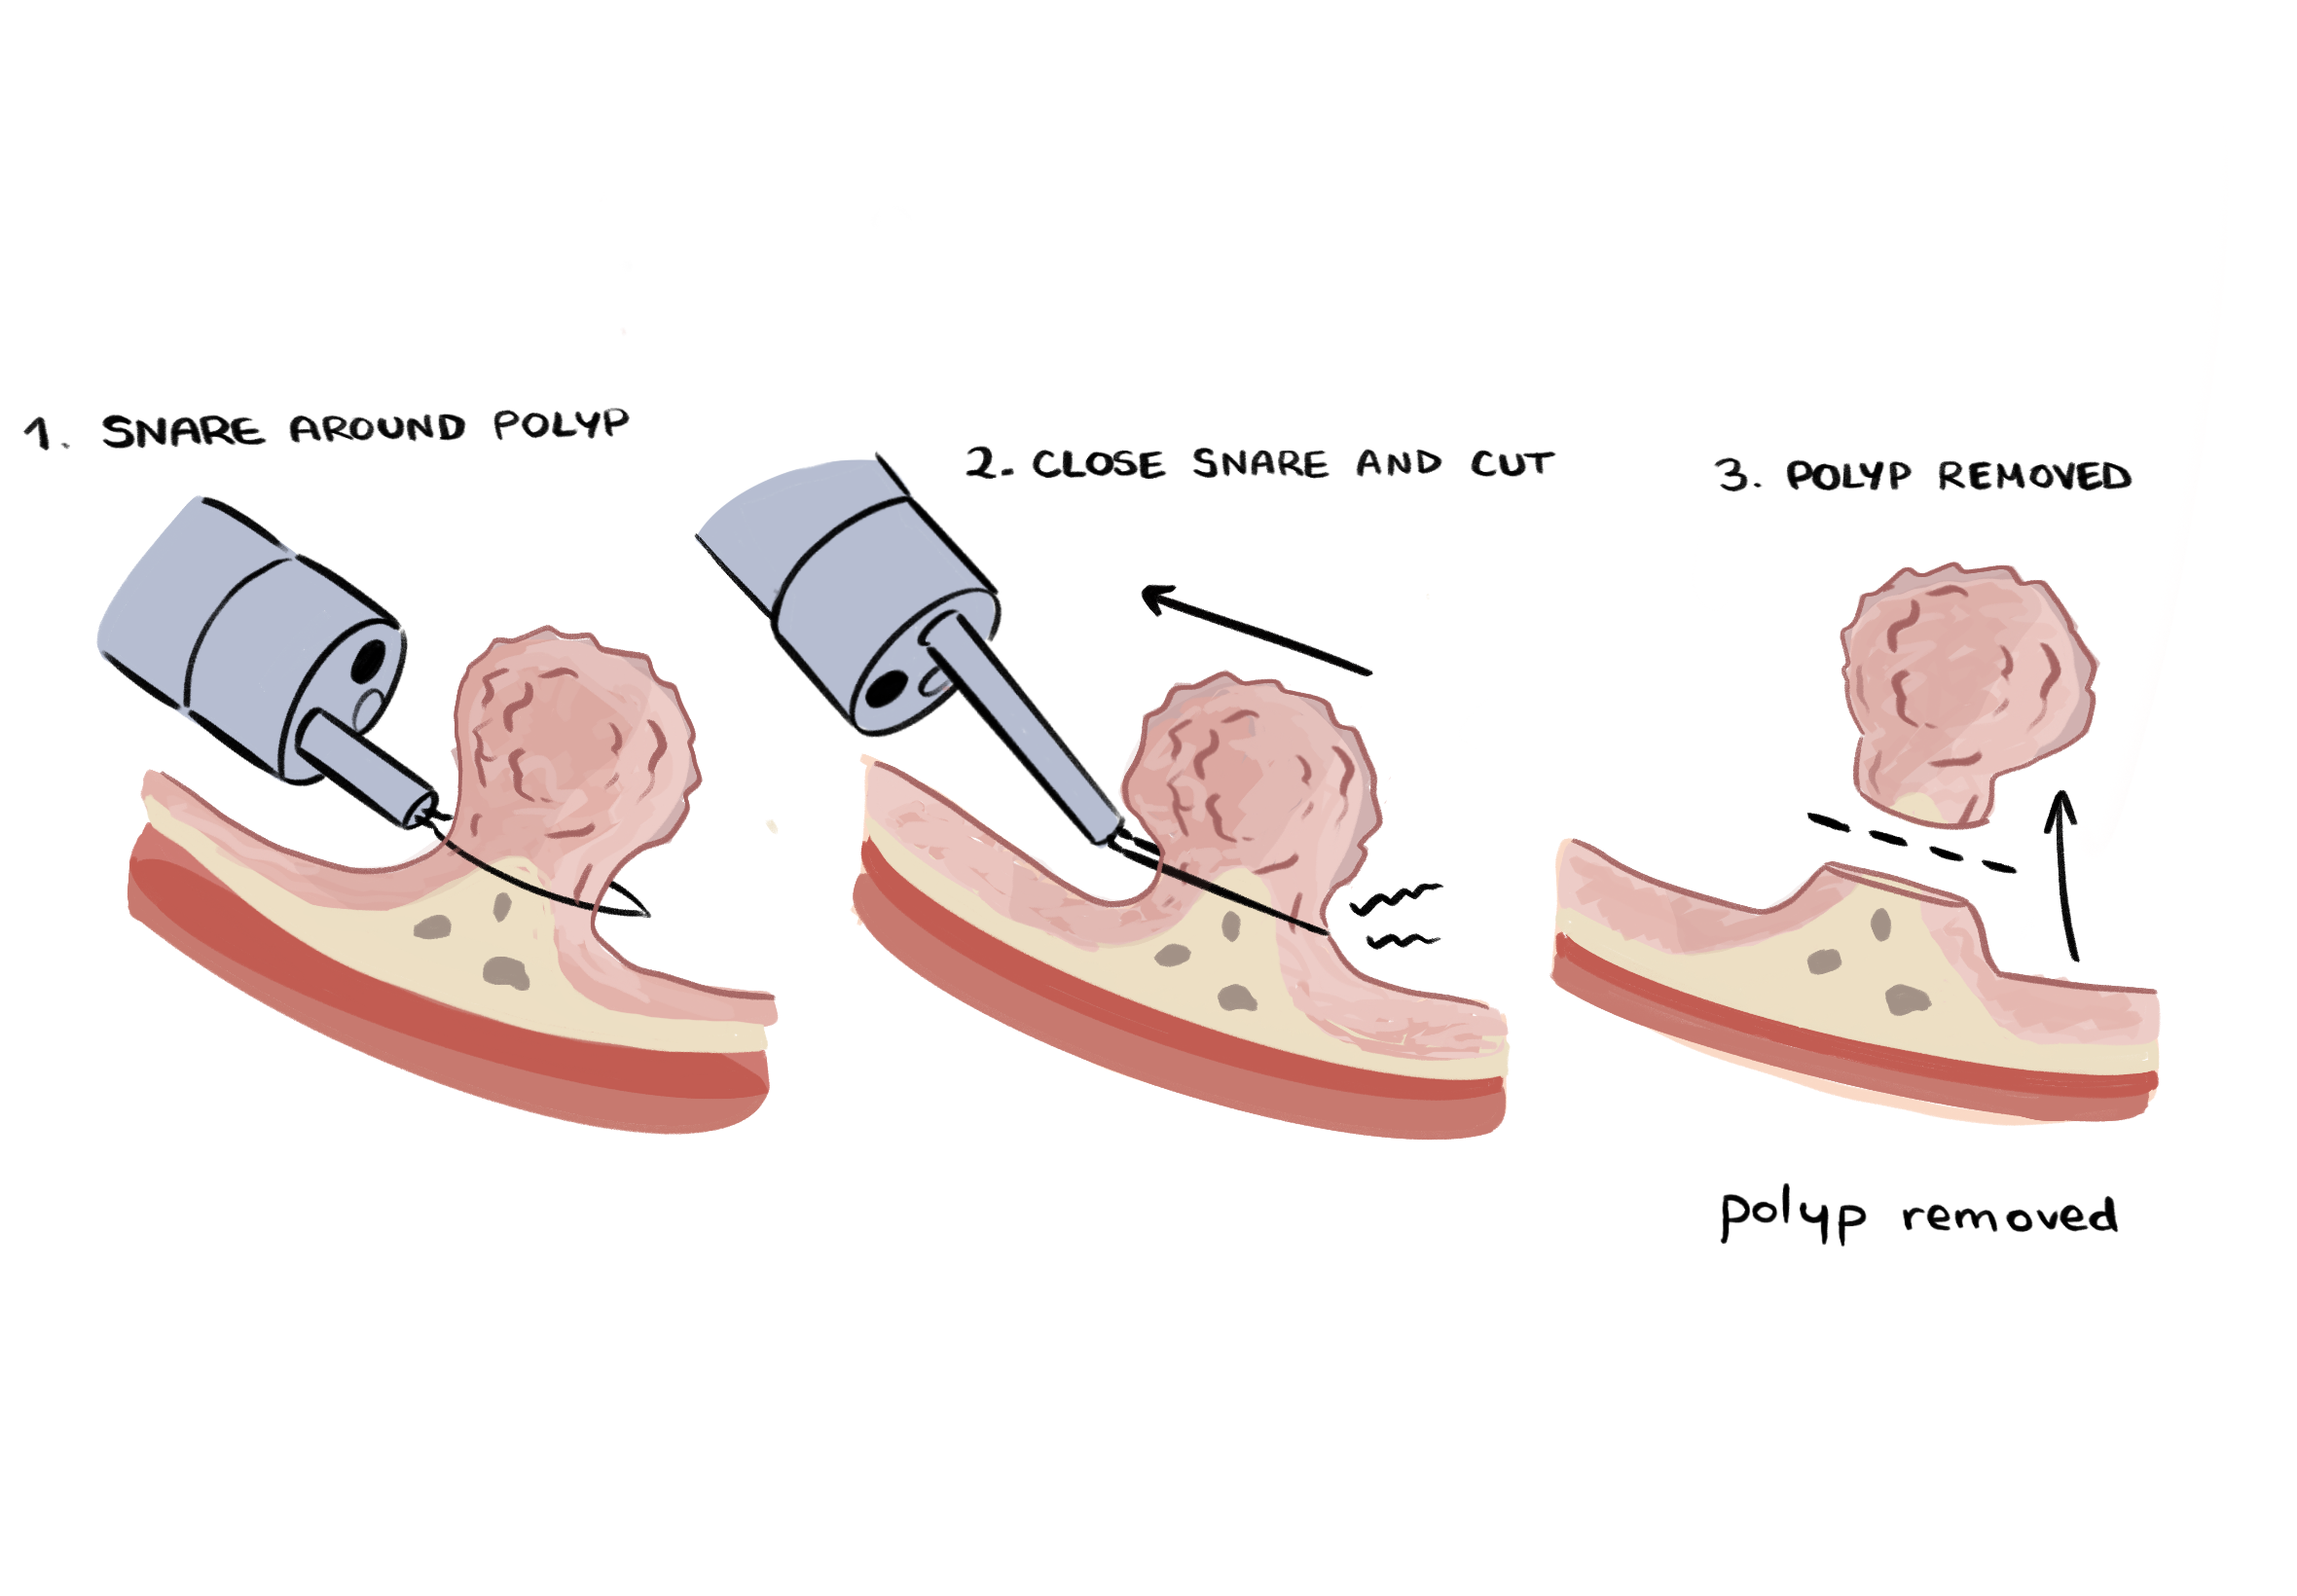
\includegraphics[width=1\linewidth,trim=0 8cm 0 3cm,clip]{assets/illustration-polyp-extraction.png}%
}
\caption{Polypectomy extraction illustration (scope tip, snare, lesion).}
\label{fig:polypectomy_extraction}
\end{figure}

After the polypectomy the operator will \textbf{inspect the site} for bleeding and check the \textbf{resection margins}. Minor bleeding is treated with \textbf{clips} or \textbf{coagulation} as needed. The patient receives brief \textbf{after-care advice} and clear instructions about signs that need urgent review.


\clearpage
Resection choice depends on lesion shape (\textbf{pedunculated} vs \textbf{sessile/flat}), size, visibility, access angle, tissue scarring, and bleeding risk \cite{ferlitsch2017esge,ESGE2024_Polypectomy_Update}.

Common options:
\begin{itemize}
\item \textbf{Cold snare}: no electrocautery; safe for small polyps and lowers thermal injury risk.
\item \textbf{Hot snare}: uses electrocautery for cutting and haemostasis; useful for some larger or bleeding lesions but adds thermal risk.
\item \textbf{Submucosal injection + snare (EMR)}: inject fluid under the lesion to lift it, then snare; good for larger sessile lesions and can be done piecemeal.
\item \textbf{ESD}: dissection in the submucosal layer for en‑bloc removal of complex lesions; offers better margins but is slower and technically demanding.
\end{itemize}


\begin{figure}[H]
\centering
\fbox{
	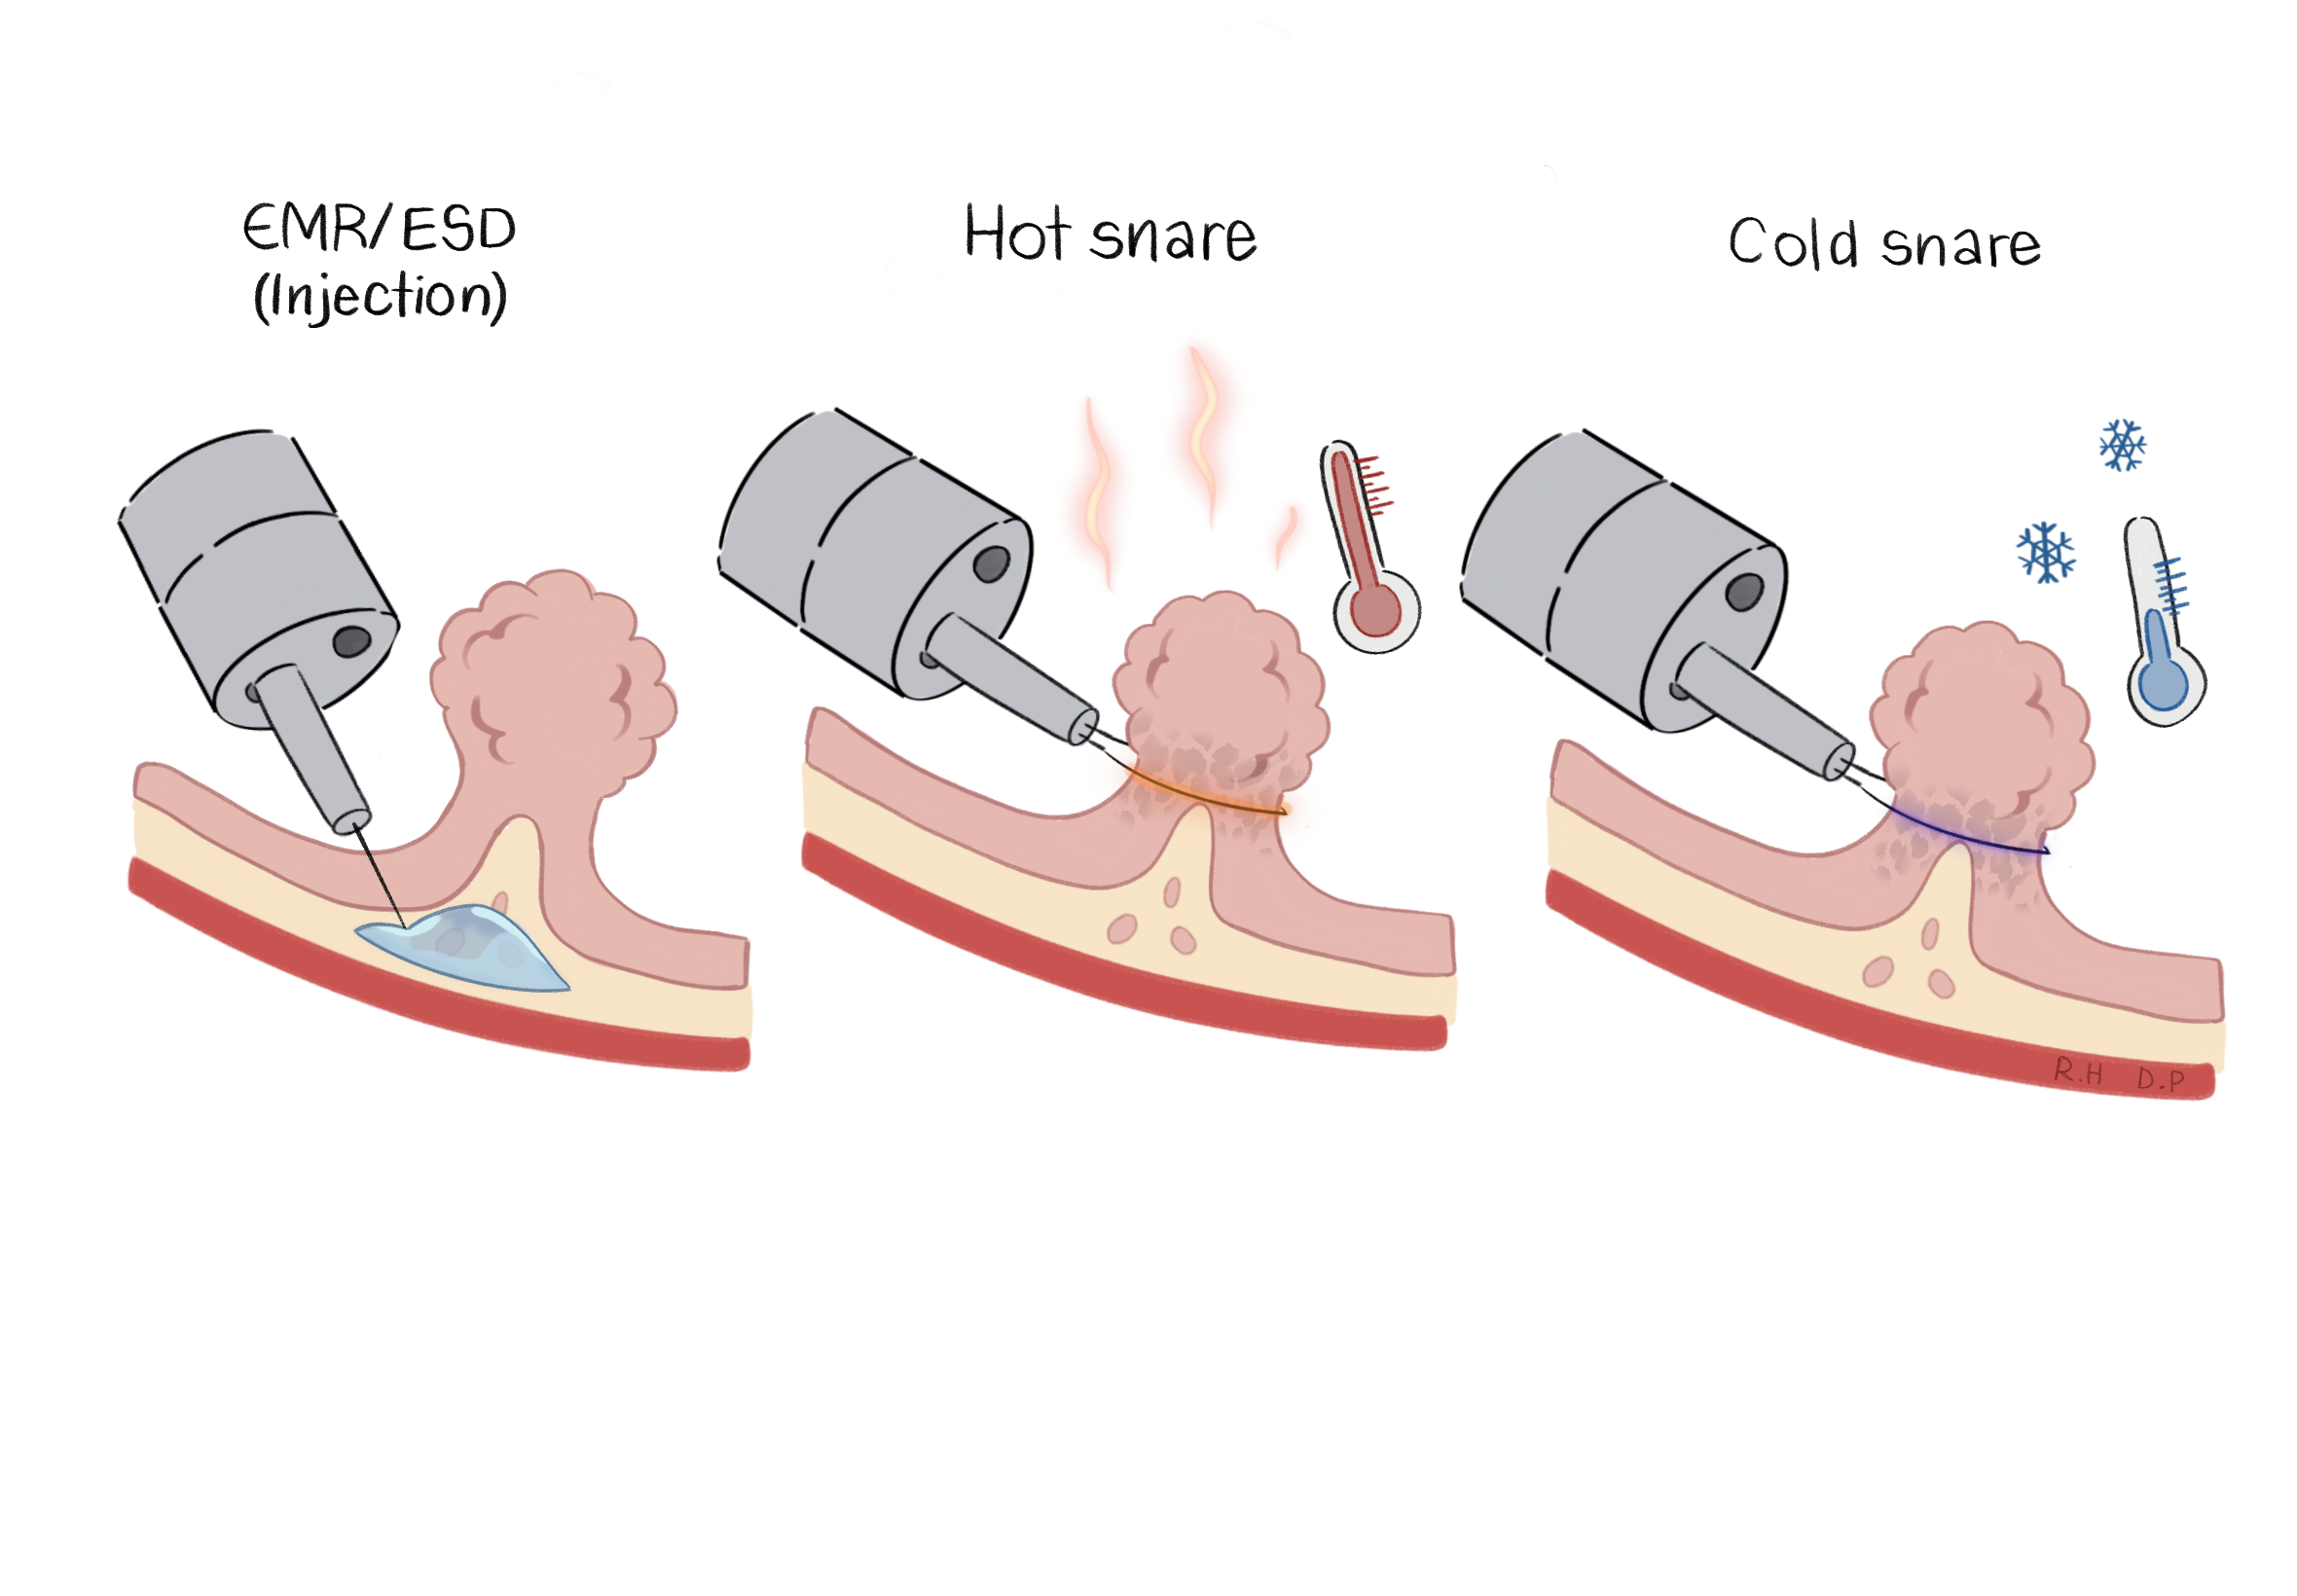
\includegraphics[width=1\linewidth,trim=0 8cm 0 3cm,clip]{assets/illustration-cutting-technique.png}%
}
\caption{Polypectomy cutting techniques (hot, cold, injection).}
\label{fig:polypectomy_cutting_techniques}
\end{figure}

When to prefer injection: if the lesion is flat or there is concern about deep invasion or scarring, a \textbf{submucosal injection} improves safety and helps achieve a clean resection plane. Cold snare is preferred for small, non‑fibrotic polyps because it reduces delayed bleeding in many trials \cite{Chang2023_AnnInternMed,Liu2023_IntJColorectalDis}.

Choosing a method balances \textbf{completeness} (low recurrence) and \textbf{procedural risk} (bleeding, perforation) and depends on operator skill. See ESGE guidance and ESD reviews for indications and technique \cite{ferlitsch2017esge,PimentelNunes2015_ESGE_ESD,ESGE2024_Polypectomy_Update}.






